\chapter{Method}\label{chap:design}
% \section{Teat Pose Estimation System Design}
\label{Background}
% 3-6 pages
% \lipsum[1]\todo{TODO}
In this chapter the different steps taken to create a 3D object detector are addressed. The following questions are answered over the course of this chapter:
\begin{itemize}
    \item How can cow teats be recognized?
    \item What are the current method's goals and limits?
    \item What is the method's pipeline composed of?
    \item What is required to apply the method?
\end{itemize}
In order to answer these questions, the structure of this chapter is illustrated as follows: Section \ref{chap:3:goal} describes the first step. It defines the computer vision task and limits its scope. Then, the choice of a suitable data set and the composition of the collected raw data is presented. Section \ref{chap:3:data} describes the information available and the choice of features for the given task. Afterwards, it describes the preprocessing of the data by identifying noise or erroneous inputs. Section \ref{chap:3:method} describes the choice of three proposed processing pipelines and the considered algorithms and techniques.  The interpretation of the performance of the algorithm is described in Section \ref{chap:3:interpretation}. This section also describes how the method results were evaluated, how the algorithms were compared to each other and which parameters were adjusted. Finally, Section \ref{chap:3:architecture} describes the architecture of the processing pipeline, illustrating the diverse components' behaviors, interactions and deployment constraints.
% dacross for determining the 3D position of the salient object. 
% It also sets out the assumptions we took and the choices of technologies with respect to what was discussed in Section 2.

% domain model
%  
\section{Identification of the Computer Vision Goal}\label{chap:3:goal}
The predefined goal of this project work was to propose a 3D object detection of cow teats solution using machine learning. As mentioned in Section \ref{chap:1:}, this project work tackles two research questions: 
\begin{itemize}
    \item How can the cow teats 3D pose and direction be estimated under 2 seconds?
    \item How can the cow teats 3D pose and direction estimation be evaluated?
\end{itemize}
To answer these questions, the following practical steps were laid out:
\begin{itemize}
    \item Conceive a computer vision processing pipeline with optimal prediction quality for identifying the 3D pose and direction of a cow teat.
    \item Present a method for evaluating the quality of the predictions regardless of the method used.
\end{itemize}
This strategy was determined because the steps for data creation and preprocessing are independent of the approach used. Therefore, the remaining task is to propose a machine-learning-enabled pipeline that solves the indicated computer vision task without a priori knowledge of the input system. The main challenge in the processing pipeline is the usage of the diverse types of information the input system provides. The method for evaluating the quality of the predictions will then be built on the results of the processing pipeline. Therefore, the computer vision task is solved by the first step and and the second one is solved by looking at the prediction outputs.

\section{Image Data}\label{chap:3:data}
In order to evaluate computer vision predictions it is essential to gather sufficient quantities of raw data and to layout a simple data structure, if required. The following questions will be answered in this section:
\begin{itemize}
    \item What kind of data is necessary?
    \item What kind of structure fulfills the requirements for the present study?
    \item What is the origin of the data?
    \item What are the preprocessing steps?
\end{itemize}
Traditional computer vision tasks require the following types of data: a training data set, for training the algorithm on the domain-specific data and a test set to determine the algorithm's prediction quality. As stated in Section \ref{chap:3:goal}, the given task is to estimate the 3D pose and direction cow teats for a cow milking robot. Therefore, the input data current accessible is: an RGB image, a depth image and a point cloud. The first attempts at tackling the problem using depth images for object classification using traditional computer vision methods failed to meet the performance criteria. Also, under the current project's conditions it is not viable to manually annotate a point cloud. It is also unfeasible to load a batch of point clouds into memory for training. Given the lack of additional inputs, each entry of the data set contains:
% to show any prediction outputs, and the execution time was over 300ms
\begin{itemize}
    \item RGB image of the cow teats.
    \item Pixel-wise segmentation mask, labeling the locations of the cow teats in the RGB image.
\end{itemize}
The collection of the data was done at a laboratory at the ZHAW. Given the limitations of the first iteration of the milking robot project, the collection of real cow images was not required. The environment setup and details of the training data collection are described in Chapter \ref{chap:evaluation}. Finally, even though since the images collected from the camera could be directly used for training, the preprocessing required was the adaptation of the data set to the COCO data format. Once formatted, the neural network could be trained.

\section{Specification of a Computer Vision Approach}\label{chap:3:method}
This section describes choice of a computer vision approach for object segmentation, the proposal of 3d pose estimation pipelines and the actual processing step. The following questions will be answered in this section:
\begin{itemize}
    \item Which and how many techniques were considered suitable for the object segmentation task?
    \item Which and how many techniques were considered suitable for the pose estimation task?
    \item How were the algorithms optimized for the data set?
    \item What were the main problems found during this phase?
\end{itemize}
Choosing the most suitable machine learning technique comes with a trade-off between the different advantages and disadvantages that each approach possesses. Therefore, multiple approaches were tested for the given task, the results analyzed and the algorithms’ parameters optimized. 

\subsection{Object Segmentation Approaches}
As described in Section \ref{chap:2:segment}, object segmentation involves the pixel-wise assignment of labels in an image that belong to a specific class. The following techniques were considered suitable for this task:
\begin{itemize}
    \item \textbf{Thresholding}
    \item \textbf{K-Means clustering}
    \item \textbf{Histogram-based image segmentation}
    \item \textbf{Edge detection}
    \item \textbf{Convolutional Neural Networks}
    \item \textbf{Fully Convolutional Networks}
\end{itemize}
The cow teat segmentation problem was tackled using two implementations of MaskRCNN: matterport/MaskRCNN and Detectron2 (FacebookAI). The evaluation and performance of both approaches is described in Section 5.

%As of 28.12.2020, MaskRCNN's repository has not been updated since 01.04.2019 and has over 1500 issues.

\subsection{Pose Estimation Approaches}
As described in Section \ref{chap:2:segment}, object segmentation involves the pixel-wise assignment of labels in an image that belong to a specific class. The following techniques were considered suitable for this task:
\begin{itemize}
    \item \textbf{Recognition of Fixed Shapes} 
    \item \textbf{Recognition of Object Classes} 
    \item \textbf{Feature-based Recognition} 
\end{itemize}
We rely on the RGB-D input received from the camera, where each image has a resolution of 640 x 480 x 4 pixels. Each pose estimation algorithm receives the input from the camera and the segmentation mask and processes it differently. 
% This was done to analyze the precision from different sources of information (for example, point cloud versus depth image).

    \subsection{Point Cloud}
    
    % !TODO
    \lipsum[2-3]
    This setup consists of the following steps:\todo{TODO}
        \begin{itemize}
        \item identify first principal component V
        \item check V's explained variance ratio > 70% (i.e., the teat is "longer than wider")
        \item transform points using PCA frames
        \item find min and max points in V direction
        \item use camera pose to find out if tip is at min/max
        \end{itemize}.
    \begin{figure}[!ht]
        \centering
        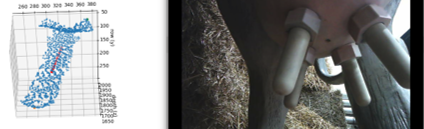
\includegraphics[width=0.8\textwidth]{images/cow_pca.png}
        \caption{A prototype of the Job Information dialog}
        \label{fig:cow_fmc}
    \end{figure}
    
    The assumptions this method makes are:
    \begin{itemize}
        \item Teats are longer than wider
        \item Tips are visible and camera angle doesn't reduce resolution in one dimension
        \item Teats point downwards
    \end{itemize}
    \lipsum[2-3]\todo{TODO}
    
    \subsection{Normals}
    
    
    \lipsum[2-3]
    This setup consists of the following steps:
        \begin{itemize}
        \item identify teat axis by minimizing sum of dot products of all normal vectors
        \item transform points using axis as principal component
        \item find min and max points in axis direction
        \item  camera pose to find out if tip is at min/max
        \end{itemize}.
    % \begin{wrapfigure}{r}{0.35\textwidth}
    %     \centering
    %     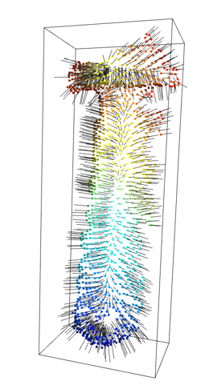
\includegraphics[width=0.2\textwidth]{images/cow_normals.png}
    %     \caption{A prototype of the Job Information dialog}
    %     \label{fig:cow_fmc}
    % \end{wrapfigure}
    
    \begin{figure}[!ht]
        \centering
        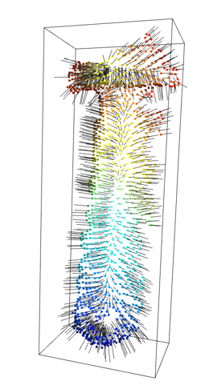
\includegraphics[width=0.2\textwidth]{images/cow_normals.png}
        \caption{A prototype of the Job Information dialog}
        \label{fig:cow_fmc}
    \end{figure}
    
    The assumptions this method makes are:
        \begin{itemize}
        \item Teat surface normals are "computable" (i.e. teat is close enough we see surface curvature)
        \item Teat is roughly cylindric in shape
        \item Tips are visible
        \item Teats point downward
        \end{itemize}
   \lipsum[2-3]\todo{TODO}

    
    \subsection{Depth Image}
    \begin{figure}[!ht]
        \centering
        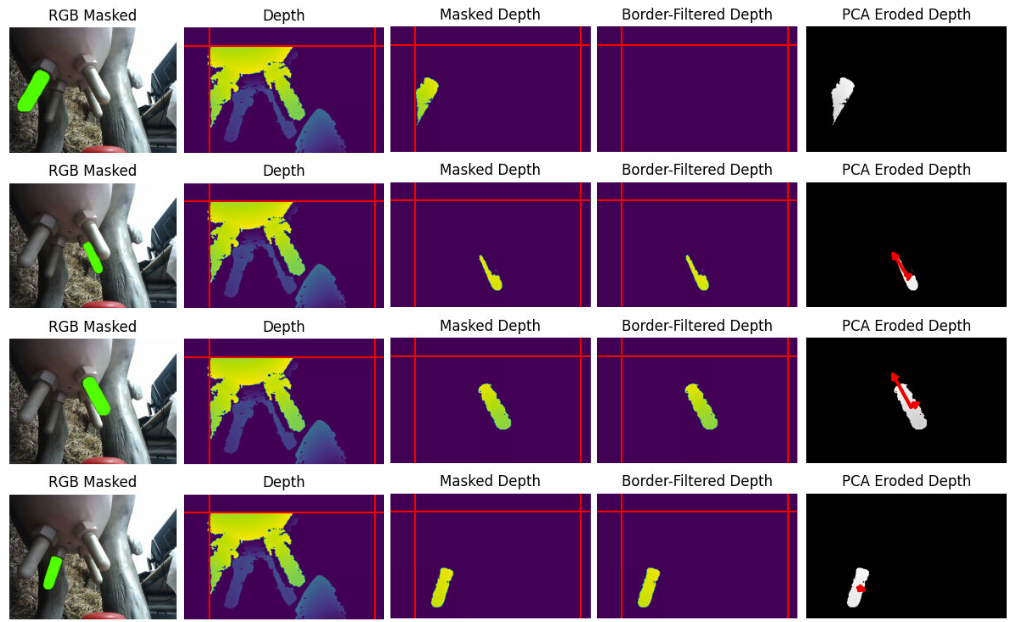
\includegraphics[width=0.7\textwidth]{images/cow_segment.png}
        \caption{A prototype of the Job Information dialog}
        \label{fig:cow_fmc}
    \end{figure}
    \lipsum[2-3]\todo{TODO}
    This setup consists of the following steps:
        \begin{itemize}
        \item RGB teat mask obtained from Detectron2
        \item Clear border-masks to avoid cut objects (rgb mask)
        \item Depth masked by the RGB mask received
        \item Clear border-masks to avoid cut objects (depth mask has different resolution)
        \item Teat width calculated from masked-depth (2D) to calculate an offset*
        \item Depth information (masked-depth) pushed to the 3D space
        \item PCA used on depth to identify teat coordinates
        \item Obtain Pose with: teat coordinates + PCA information 
        \item 4-queue structure with "memory", used to manipulate, organize and filter Poses
        \end{itemize}
    
    The assumptions this method makes are:
        \begin{itemize}
            \item Teats are longer than wider
            \item Tips are visible and camera angle doesn't reduce resolution in one dimension
            \item Teats point downward
            \item Depending on memory of queues, the algorithm can adapt quickly or slowly to new teats (timestamp filtering on the backlog)
        \end{itemize}
    \lipsum[2]\todo{TODO}
    
    While the baseline approach using just a CNN is not even in theory capable of accumulating enough
information of the scene to answer all questions posed in section 3.1, it is instead much easier to
train a neural network which does not use image sequences but independent images only as input, due
to its lower dimensionality. Each architecture setup is composed from a number of sub-networks for
better reusability. The CNN + RNN version for example uses the same feature extraction layer as the
baseline version and all three setups rely on the same number of fully connected layers for creating the
scene embedding vector. 
% The backpropagation of error is performed end-to-end through all different sub-networks. The streams that output information regarding a single object are evaluated multiple times on each timestep using randomly selected objects and their loss is accumulated. The enumerating stream which is designed to output all objects is evaluated once each frame.
The performance evaluation of these algorithms is described in Chapter \ref{chap:evaluation}.

\section{Interpretation}\label{chap:3:interpretation}

\section{Processing Pipeline Design}\label{chap:3:architecture}
% \section{Software Design} 
% \section{FMC Diagram}
The Fundamental Modeling Concepts (FMC) provide a framework for the comprehensive description of software-intensive systems. 
% Its block diagrams show the compositional structures as a composition of collaborating system components.
Active system components are called agents and passive system components are called locations (storage, channels, queues; where information can be observed) \cite{FMCdiag}. The following FMC diagram (Figure \ref{fig:cow_fmc}) describes the high-level overview of the system's architecture.
    \begin{figure}[!ht]
        \centering
        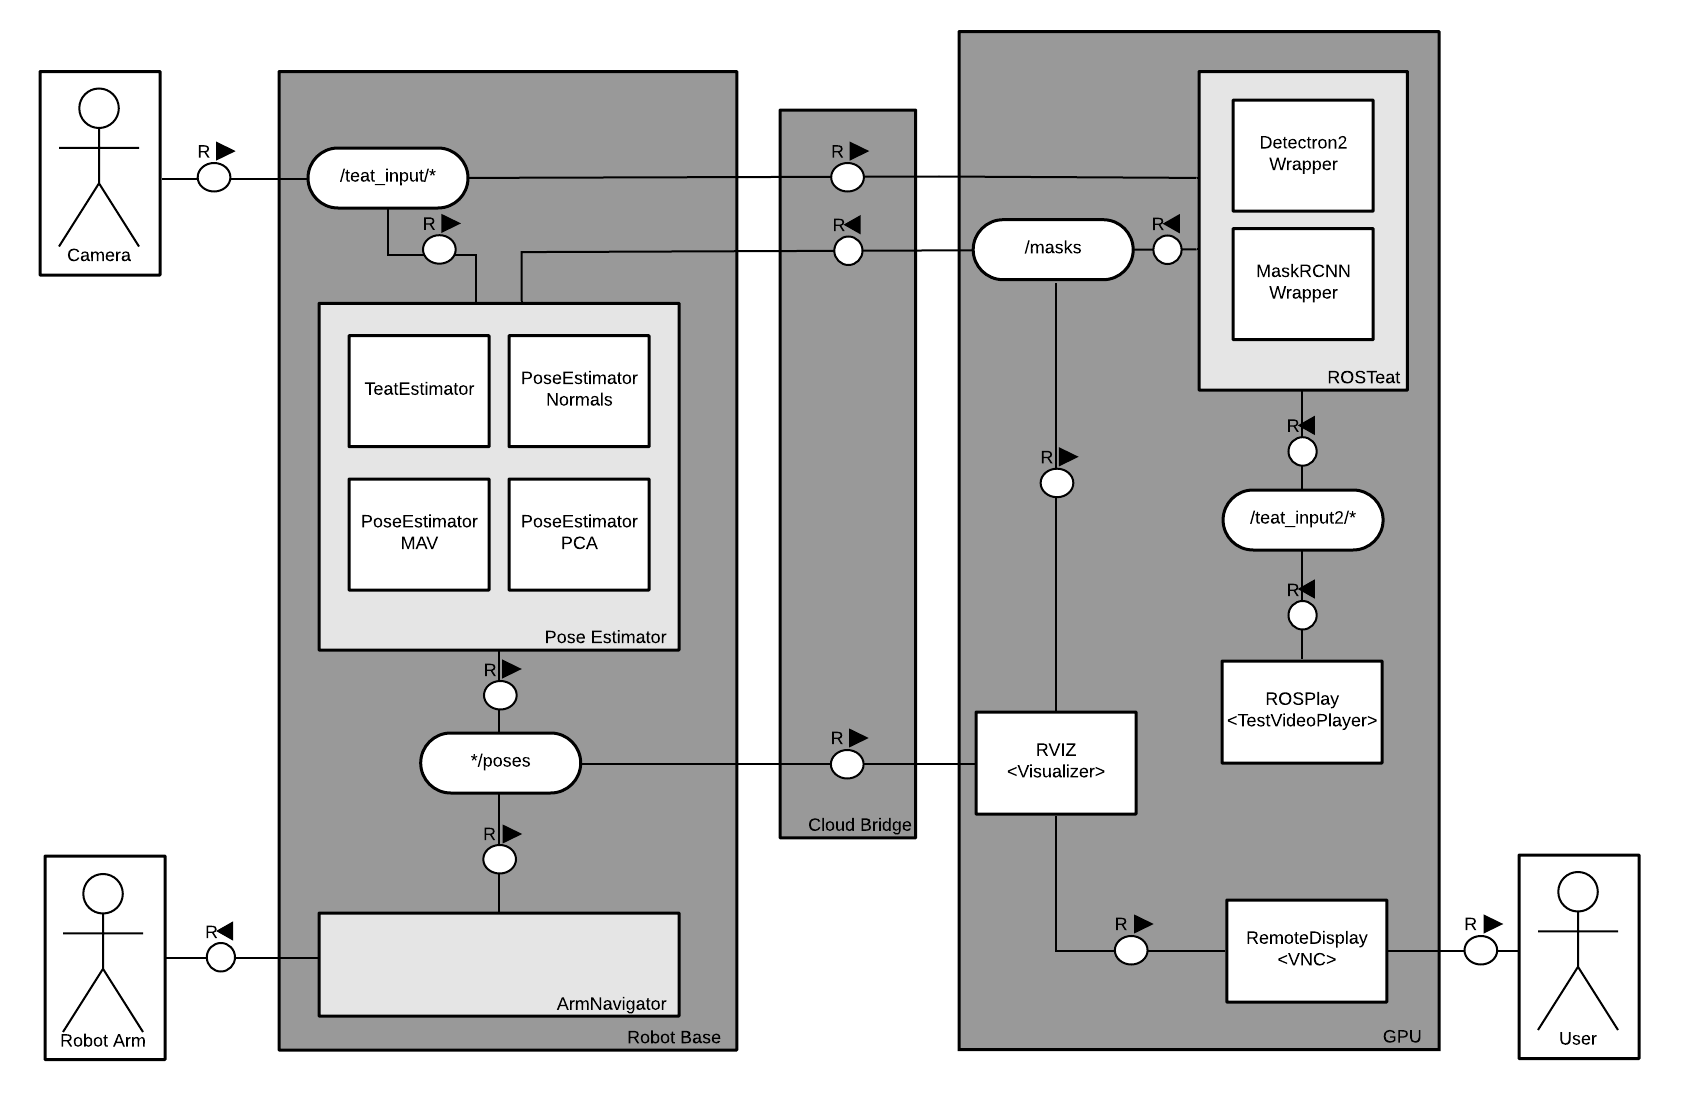
\includegraphics[width=1\textwidth]{images/cow_fmc.png}
        \caption{A prototype of the Job Information dialog}
        \label{fig:cow_fmc}
    \end{figure}
    
% \newpage
\lipsum[2]\todo{TODO}
The FMC diagram in Figure \ref{fig:cow_fmc} describes the following agents and locations:
\begin{itemize}
    \item \textbf{Camera:} captures frames and publishes these as input for all the other components.
    \item \textbf{User:} uses Rviz to visualize: the point cloud, the RGB image, the depth image, the segmented image of the cow teats and the 3D poses published.
    \item \textbf{Robot Arm:} moves according to the instructions given by ArmNavigator. 
    \item \textbf{PoseEstimator:} pose estimation algorithm that processes the information received from the camera and ROSTeat to predict 3D poses.
    \item \textbf{ROSTeat Node:} processes images from the Camera node and segments the cow teats in the image.
    \item \textbf{ArmNavigator:} manipulates the RobotArm according to the 3D poses published.
    \item \textbf{ROSPlay <TestVideoPlayer> Node:} Behaves as a simulation/testing mechanism for reproducing the camera videos.
    \item \textbf{RVIZ <Visualizer>:} ROS framework that allows the visualization of different ROS topics (RGB image, point cloud, etc.)
    \item \textbf{RemoteDisplay <VNC>:} this is a browser-based graphical-d
    esktop system that allows the visualization of RVIZ.
    \item \textbf{/teat input/*:} channel where the camera input is published for other components to consume.
    \item \textbf{/teat input2/*:} channel where the simulation video is published as input for other components to consume.
    \item \textbf{/masks:} channel where the segmented cow teats are published.
    \item \textbf{*/poses:} channel wehre the 3D cow teat poses are published.
\end{itemize}

The behavior and interactions of the main components (ROSTeat and Pose Estimator) are described in the following sections with more detail.

\subsection{Use Cases}
\lipsum[2]\todo{TODO}
\begin{longtable}{@{} p{3.5cm} p{10.5cm} @{}} \toprule
\textbf{Use Case}       & \textbf{Predict Cow Teat Masks} \\ \midrule
Actor                   & ROSTeat Node \\ \cmidrule{1-2}
Description             & A cow teat is recognized from an image. \\ \cmidrule{1-2}
Goal                    & Publish the cow teat masks present in received image. \\ \cmidrule{1-2}
Preconditions           & An image exists. \\ 
                        & ROSTeat node is running. \\ \cmidrule{1-2} 
Postconditions          & A number of masks have been identified from image [0+]\\ \cmidrule{1-2} 
                        & 1. The camera publishes an image. \\ 
Basic Flow              & 2. The ROSTeat node consumes the image and predicts the cow teats in it. \\
                        & 3. The ROSTeat node publishes the masks for future processing. \\ \cmidrule{1-2}
Exceptions             & Image is not RGB \\ \bottomrule
\caption{Use Case - Predict Masks} \label{tab:tabcu-prop} \\
\end{longtable}

% \newpage
\begin{longtable}{@{} p{3.5cm} p{10.5cm} @{}} \toprule
\textbf{Use Case}       & \textbf{Estimate Cow Teat Pose} \\ \midrule
Actor                   & Pose Estimator \\ \cmidrule{1-2}
Description             & A cow teat pose is recognized from a tuple (image, point cloud, depth image, mask). \\ \cmidrule{1-2}
Goal                    & Publish the cow teat poses for each message received. \\ \cmidrule{1-2}
Preconditions           & An image exists. \\ 
                        & ROSTeat node is running. \\ \cmidrule{1-2} 
Postconditions          & A number of cow teat poses have been identified from image [0+]\\ \cmidrule{1-2} 
                        & 1. The camera publishes an image AND ROSTeat node publishes the masks for the image (synchronized receival, stored as a tuple). \\ 
Basic Flow              & 2. The Pose Estimator node consumes the tuple and predicts the cow teat poses in it. \\
                        & 3. The Pose Estimator node publishes the poses for posterior attachment. \\ \cmidrule{1-2}
Exceptions             & TransformListener is empty \\ 
                       & Any element in the tuple is empty and masks are not (data corruption). \\ \bottomrule
\caption{Use Case - Predict Poses} \label{tab:tabcu-prop} \\
\end{longtable}
\lipsum[2]\todo{TODO}

